\documentclass[RNAAS]{aastex631}
\usepackage{graphicx}
\usepackage{placeins}

\shorttitle{HD 170312, a long-period eclipsing binary}
\shortauthors{Meneguzzo}

\begin{document}

\title{HD 170312 is a bright, long-period eclipsing binary}

\author[0009-0000-0032-3262]{Mauri de Souza Meneguzzo}
\affiliation{Independent researcher}

\begin{abstract}
I identify HD 170312 ($V=8.7$), an evolved F star, as a long-period eclipsing binary. TESS shows four eclipses centered on the star, two 8.5 and two 15.4 percent deep; the fourth lies in cadences flagged for scattered light. Only two orbital periods fit them, 137.90 and 68.95\,d. A possible egress in sector 101, a NEOWISE visit of 2014 and ASAS-3 photometry favor 68.95\,d. A deep eclipse on 2027 March 11 (BTJD 4475.8152), in TESS sector 114, would settle the period.
\end{abstract}

\keywords{Eclipsing binary stars (444) --- Stellar photometry (1620) --- Light curves (918)}

\section*{}

I report an eclipsing binary that had not been recognized: HD 170312 (TIC 292292315; F3\,IV/V, $V=8.71$; \citealt{Stassun2019}). No catalog I searched lists it as variable, including the TESS eclipsing binary catalog \citep{Prsa2022} and the Gaia DR3 variability tables \citep{GaiaMission,GaiaDR3}. I call the F star A and its companion B.

The star was found by a search of multi-sector TESS 2-minute light curves \citep{Ricker2015,Jenkins2016} with transitgpu 0.4.0 \citep{Meneguzzo2026}. Its peak, at 12.9\,d $=1792.694/139$\,d, is a spacing of the eclipses, not the orbital period.

TESS recorded four complete eclipses (Figure~1b). Three lie in unflagged data, in sectors 39, 102 and 103, at BTJD $2377.1543\pm0.0002$, $4131.0663\pm0.0001$ and $4169.8482\pm0.0005$. The first and third are 8.5 percent deep and the second 15.4 percent, each uncertain by about 1.5 percentage points because the PDC correction tilts the baseline beside the sector 102 eclipse.

The fourth eclipse lies in 715 flagged cadences that continue sector 93 for a day, 359 of them flagged for scattered light, which PDCSAP omits. Their SAP flux holds a deep eclipse. Fitted with the shape of the sector 102 eclipse, it is centered at BTJD 3855.2675, 20\,s from the predicted time, at 1.003 times that eclipse's depth. It is the star's, not the scattered light's: the fall in each of 121 pixels is proportional to that pixel's light out of eclipse (correlation $-0.998$), and the depth changes by under 0.1 percentage point across five background estimates, although the background rises more than tenfold.

The eclipses come from the HD 170312 system. The dimming lies within $2.2''$ of A, and every Gaia DR3 source within $5''$ is $G=19.6$ or fainter, 11 magnitudes too faint to make a 15 percent dip.

B is a star, too large for a planet or a brown dwarf. As I do not know which eclipse has B in front of A, the shallow one bounds its size: $R_B\geq R_A\sqrt{\delta/c}$, where $c=1.134$ is the ratio of the central to the mean intensity of A for quadratic limb darkening at 6645\,K and $\log g=3.5$ \citep{Claret2017}. This gives $R_B\geq0.95\,R_\odot$ with the TIC radius $R_A=3.46\,R_\odot$. Two-star models fitted to the eclipses need A to be 24 to 34 percent smaller than its TIC radius, which I cannot explain; with their smallest $R_A$, $2.27\,R_\odot$, $R_B\geq0.62\,R_\odot$.

Two periods fit the four eclipses. The shallow eclipses are $\Delta T=1792.694$\,d apart, so each kind recurs with $P=\Delta T/N$ for an integer $N$. Of 3,200 values of $N$, only $N=13$ and 26 ($P=137.90$ and 68.95\,d) predict all four eclipses and none where the data show none. The eclipses only 68.95\,d predicts fall in gaps of the TESS coverage, except at the start of sector 101 (Figure~1a). The two-star models fit both periods equally well. The deep eclipse falls at phase 0.44 of the 68.95\,d orbit or 0.72 of the 137.90\,d one, so the orbit is eccentric, with $e\geq0.10$ or 0.34.

Three observations favor 68.95\,d. First, flagged cadences at the start of sector 101 rise as the egress of a shallow eclipse at the time only 68.95\,d predicts (BTJD 4100.898), at 0.997 times that eclipse's depth (Figure~1b). Five similar stars on the same CCD show no such rise, two brighter ones show ramps there, and the event was examined after the data were seen. Second, ASAS-3 observed the star every two days from 2000 to 2009 \citep{Pojmanski1997}. On the ten nights only 68.95\,d places in eclipse, a test fixed before it was run, but after its points were examined, finds the star fainter by 1.04 times the TESS depths ($p\approx0.01$ over shifts of the ephemeris; Figure~1c). Each deficit is a single point, so ASAS-3 leans toward 68.95\,d without deciding. Third, a NEOWISE visit \citep{Mainzer2014} on 2014 September 24 covers the deep eclipse only 68.95\,d predicts: the star fades by 0.13\,mag in W2, faintest at the predicted time within the 95 minutes between exposures, while none of 11 stars in the same frames, one as bright, fades by more than 0.02\,mag. The visit has no control eclipse and was found after the period analysis, so it favors 68.95\,d without establishing it. ASAS-SN photometry of 2014 to 2026 \citep{Shappee2014,Kochanek2017,Winecki2024} is fainter at the eclipses both periods predict, by 2.07 times the TESS depths ($p<5\times10^{-5}$), but not at those only 68.95\,d predicts ($0.89\pm0.37$ times).

The period can be tested on 2026 December 2, when only 68.95\,d predicts a shallow eclipse, and settled on 2027 March 11 by a deep eclipse at BTJD $4475.8152\pm0.0002$, which TESS sector 114 covers and 137.90\,d does not predict. The classification rests on photometry: I found no public spectrum, and Gaia DR3 gives no radial velocity.

\begin{figure}[ht]
\centering
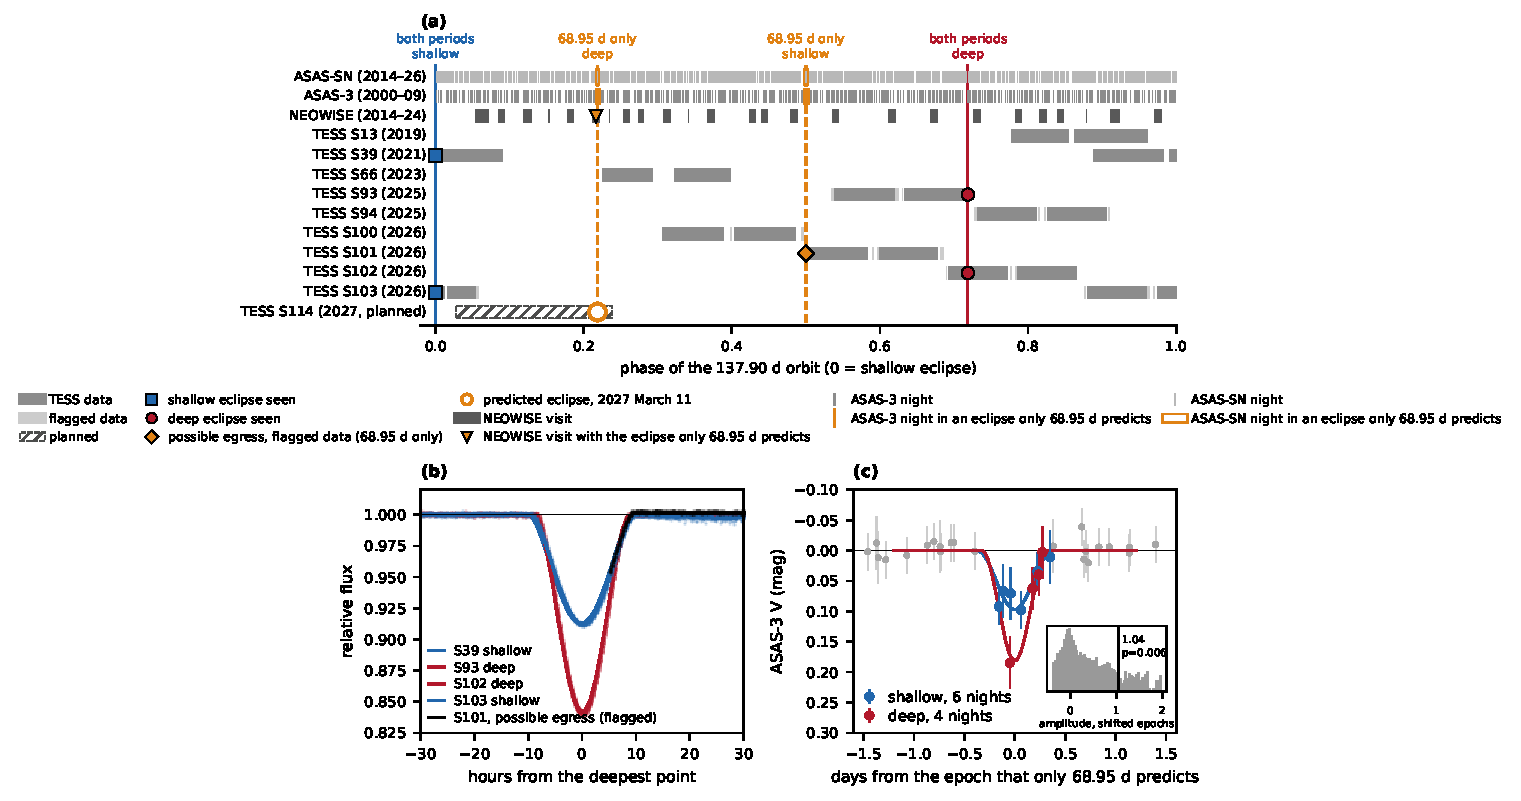
\includegraphics[width=0.95\columnwidth]{figures/events.pdf}
\caption{(a) Phases of the 137.90\,d orbit (0 at the shallow eclipse) covered by each TESS sector and, in the top rows, by ASAS-SN, ASAS-3 and NEOWISE. Solid lines: shallow (blue) and deep (red) eclipses both periods predict; dashed orange: those only 68.95\,d predicts. Orange ticks mark the ASAS-3 nights of (c), the triangle the NEOWISE visit, hollow boxes the ASAS-SN nights in those windows. Marks show coverage, not fading; markers show the eclipses seen, the possible egress of sector 101 and the eclipse of 2027 March 11. (b) The four eclipses in SAP flux, 1\,h medians, aligned on minimum; black, the flagged start of sector 101. (c) ASAS-3 nightly V means on the ten nights and, in grey, other nights, with the TESS eclipse shapes; errors scaled by 2.9 to the data's scatter. Inset: amplitudes at 20,000 shifted epochs; 0.6 percent reach the fitted 1.04.}
\end{figure}

\FloatBarrier
\begin{acknowledgments}
This paper uses TESS data from the MAST archive at STScI (doi:10.17909/t9-nmc8-f686), which is operated by AURA under NASA contract NAS5--26555; TESS is funded by the NASA Explorer Program. It uses data products of NEOWISE (doi:10.26131/IRSA144), a project of JPL/Caltech funded by NASA, and the SIMBAD database. This work has made use of data from the European Space Agency (ESA) mission {\it Gaia} (\url{https://www.cosmos.esa.int/gaia}), processed by the {\it Gaia} Data Processing and Analysis Consortium (DPAC, \url{https://www.cosmos.esa.int/web/gaia/dpac/consortium}). Funding for the DPAC has been provided by national institutions, in particular the institutions participating in the {\it Gaia} Multilateral Agreement. An AI language model (Anthropic Claude) assisted with the code and the writing.
\end{acknowledgments}

\begin{thebibliography}{13}
\bibitem[Claret(2017)]{Claret2017} Claret, A. 2017, A\&A, 600, A30
\bibitem[Gaia Collaboration(2016)]{GaiaMission} Gaia Collaboration, Prusti, T., de Bruijne, J. H. J., et al. 2016, A\&A, 595, A1
\bibitem[Gaia Collaboration(2023)]{GaiaDR3} Gaia Collaboration, Vallenari, A., Brown, A. G. A., et al. 2023, A\&A, 674, A1
\bibitem[Jenkins et al.(2016)]{Jenkins2016} Jenkins, J. M., Twicken, J. D., McCauliff, S., et al. 2016, Proc. SPIE, 9913, 99133E
\bibitem[Kochanek et al.(2017)]{Kochanek2017} Kochanek, C. S., Shappee, B. J., Stanek, K. Z., et al. 2017, PASP, 129, 104502
\bibitem[Mainzer et al.(2014)]{Mainzer2014} Mainzer, A., Bauer, J., Cutri, R. M., et al. 2014, ApJ, 792, 30
\bibitem[Meneguzzo(2026)]{Meneguzzo2026} Meneguzzo, M. de S. 2026, Parallel Search for Alien Worlds: GPU-Accelerated BLS and TLS for Exoplanet Transit Detection, preprint, github.com/mauri870/transitgpu
\bibitem[Pojmanski(1997)]{Pojmanski1997} Pojmanski, G. 1997, Acta Astron., 47, 467
\bibitem[Pr\v{s}a et al.(2022)]{Prsa2022} Pr\v{s}a, A., Kochoska, A., Conroy, K. E., et al. 2022, ApJS, 258, 16
\bibitem[Ricker et al.(2015)]{Ricker2015} Ricker, G. R., Winn, J. N., Vanderspek, R., et al. 2015, JATIS, 1, 014003
\bibitem[Shappee et al.(2014)]{Shappee2014} Shappee, B. J., Prieto, J. L., Grupe, D., et al. 2014, ApJ, 788, 48
\bibitem[Stassun et al.(2019)]{Stassun2019} Stassun, K. G., Oelkers, R. J., Paegert, M., et al. 2019, AJ, 158, 138
\bibitem[Winecki \& Kochanek(2024)]{Winecki2024} Winecki, D., \& Kochanek, C. S. 2024, ApJ, 971, 61
\end{thebibliography}

\end{document}
